\chapter{Partie réseau}
	\section{Transmission des données et protocole}
	L'ensemble des classes spécifiques au réseau est regroupé dans le package network. Deux classes séparés permettent de différencier la partie serveur (qui héberge la partie) de la partie client (qui communique uniquement avec serveur).

	Le serveur enregistre la liste des joueurs et donne la main à l'un d'entre eux grâce à la classe PlayerManager. Cette dernière contient un tableau dans lequel les joueurs sont classés dans l'ordre des propositions qu'ils ont réalisé. A chaque fois qu'un joueur passe la main, le compteur de cette classe s'incrémente pour accéder à la case suivante. Le joueur qui a la main en premier est celui qui a fait la plus petite proposition et le plus rapidement (première case du tableau).

	Les données sont formatés à l'aide de la classe protocol qui permet d'encoder et de décoder les différents messages qui sont transmis sous forme de chaîne de caractère (String). Des préfixes au début de chaque message permettent de déterminer quel type de données sont transmises. Les préfixes et données sont séparés au sein d'un même message par un caractère séparateur (typiquement le symbole \&).

	\vspace{0.5cm}
	Exemple :
	\begin{verbatim}
	String robotInfo = ROBOT + "&" + r.x + 
	                           "&" + r.y + 
	                           "&" + r.getColor() + 
	                           "&" + r.originX +
	                           "&" + r.originY;
	\end{verbatim}
    
	\section{Caractéristiques techniques}
	Notre application fonctionne uniquement sur un réseau local avec des adresses du type IPv4. En effet, la plupart du temps sur Internet l'utilisateur se trouve derrière un routeur (une box), il ne nous est pas possible de le gérer à notre niveau. Le port utilisé par le serveur (3001) et différent du port utilisé par le client (3002), cela nous a notamment permis de tester avec une seule machine (en localhost avec l'adresse 127.0.0.1).

	\begin{figure}[h!]
   	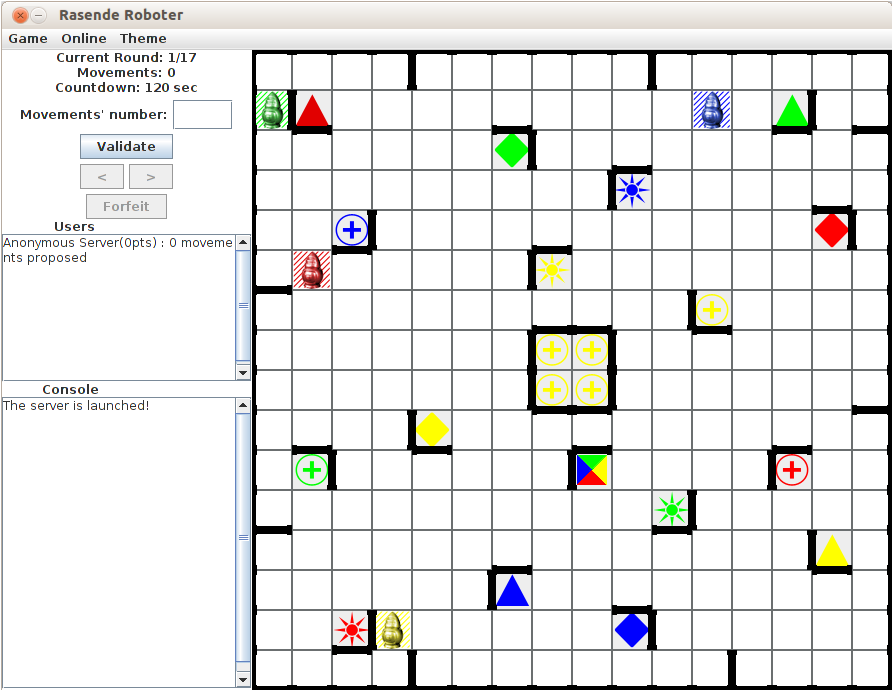
\includegraphics[scale=0.45]{img/multi.png}
	\caption{Vue d'une partie en réseau, avec la colonne de droite qui contient des données supplmentaires par rapport au solo (liste des joueurs, bouton pour déclarer forfait, ...)}
	\end{figure}
	
\newpage
	\section{Glossaire du protocole}
	Liste des préfixes possibles dans le protocole avec les explications sur le type de message transmit à leur suite :
\vspace*{5mm}
	\begin{itemize}
	\item[-] BOARD\_PIECE : envoie l'adresse du quart du fichier xml contenant le plateau à charger et la position où le mettre.
	\item[-] BUTTON\_VALIDATE : permet de dire si le bouton "validate" est actif ou non.
	\item[-] CLIENT : permet d'envoyer la liste des joueurs et leurs données (pseudo, points...) pour l'affichage dans la colonne latérale.
	\item[-] CONNECT : nouvelle connexion entre un client et un serveur.
	\item[-] GOAL\_CARDS : envoie la pile des cases à atteindre.
	\item[-] HAND : permet d'envoyer un message indiquant à un joueur qu'il prend ou perd la main.
	\item[-] MESSAGE : pour transmettre un message à tous, qui s'affichera dans la console latérale du jeu.
	\item[-] MOVE : pour transmettre la position de l'ensemble des robots et le tour courant après un mouvement.
	\item[-] NEXTPROPOSITION : envoyée si un joueur passe la main, permet de demander au serveur de la donner à quelqu'un d'autre
	\item[-] OTHER\_USERNAME : appelé lorsqu'un client essaie de se connecter avec un pseudo déjà pris.
	\item[-] PROPOSITION : permet au client d'envoyer une proposition du nombre de mouvement au serveur.
	\item[-] ROBOT : transmet les données d'un robots au chargement du jeu.
	\item[-] SERVER\_DISCONNECT : permet d'informer les clients que le serveur n'est plus en ligne.
	\item[-] TIME : permet d'envoyer la mise à jour du compte à rebours.
	\end{itemize}

\vspace*{5mm}
	Ce protocole doit être étoffé pour résoudre encore certains problèmes qui apparaissent en réseau, nous n'avons par exemple pas géré le cas d'un client qui se déconnecterait (préfixe possible du message : CLIENT\_DISCONNECT), le server doit dans ce cas le retirer de sa liste et en informer tous les autres clients en mettant à jour leurs listes respectives (en renvoyant un message du type CLIENT).



